\begin{enigme}[Vitraux de cathédrales]

Dans les deux cas construis un carré de côté 6 cm :

\begin{minipage}[c]{0.3\linewidth}
\end{minipage}\hfill %
\begin{minipage}[c]{0.2\linewidth}
\centering

\includegraphics[width=2.8cm]{vitre}
\end{minipage} \hfill %
\begin{minipage}[c]{0.2\linewidth}
\centering

\includegraphics[width=1.9cm]{rosace}
\end{minipage} \hfill %
\begin{minipage}[c]{0.3\linewidth}
\end{minipage} 


\underline{Programme de construction} :
\begin{itemize}
 \item Construis un arc de cercle de centre A et de rayon AE ; il coupe [AC] en un point que tu nommeras I ;
 \item Construis le point J tel que le quadrilatère AEJI soit un losange ;
 \item Nomme K le point d'intersection de la diagonale [AJ] et du segment [EG].
                
Trace le cercle de centre K passant par E ;
 \item Place les points L et N sur le segment [HF] tel que LF = EK = HN ;
 \item Trace le cercle de centre L passant par F et celui de centre N passant par H ;
 \item Place le point M sur le segment [EG] tel que MG = EK ;
 \item Trace le cercle de centre M passant par G.
 \end{itemize}
Tu obtiens ainsi une rosace à quatre branches que tu peux voir dans certaines églises.
 
 \end{enigme}
 
 \vspace*{2em}
 
%%%%%%%%%%%%%%%%%%%%%%%%%%%%%%%%%%%%%%%%%%%%%%%%%%%%%%%%%%%%%%%%%%%%%

\begin{enigme}[L'art de l'islam]

\begin{center}
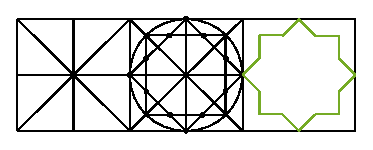
\includegraphics[width=5.4cm]{islam}
\end{center}

Tu peux réaliser une belle frise avec ce motif.
\end{enigme} 
